\section{Planificación}
Esta sección contiene las diferentes etapas del desarrollo, indicando de manera
detallada el periodo que ocupa cada una en el plano general, las horas
invertidas en cada una y los objetivos alcanzados.

Debido a la naturaleza secuencial del desarrollo, se han dividido todas las
etapas en diferentes fases, en primer lugar se encuentran las fases previas al
desarrollo, investigando el contexto del proyecto y el estado de la cuestión. En
segundo lugar se encuentran las diferentes fases del desarrollo, algunas de las
cuales precedidas por una pequeña fase de investigación en la que se
investigaban los conceptos relacionados con las tecnologías a implementar en la
fase que la sigue. En último lugar se encuentra una fase de validación general y
el estudio final:
\begin{itemize}
    \item \textbf{Análisis de contexto y proyecto}: Durante esta primera fase se
    exploró todo el entorno relacionado con el proyecto, realizando un estudio
    sobre los objetivos de desarrollo sostenible, explorando todo el contexto al
    rededor de los mismos y su importancia en la sociedad moderna.
  
    \item \textbf{Investigación del estado del arte}: Esta segunda fase se
    centro en el estudio del estado del arte, analizando las múltiples
    soluciones similares existentes y sus características principales.
    Adicionalmente se realizó un estudio sobre las diferentes arquitecturas y
    teoría relacionada con las redes de neronas 
    
    \item \textbf{Iteración inicial}: Esta primera fase de desarrollo esta
    formada por tres etapas diferentes la primera de ellas consiste en una
    búsqueda de datos que usar para el entrenamiento. Esta esta continuada por
    la generación y entrenamiento de una serie de modelos que finalmente fueron
    sometidos a una fase de validación y pruebas para analizar el progreso
    conseguido.
   
    \item \textbf{investigación segunda iteración}: en la segunda iteración se
    decidió implementar una arquitectura nueva, basada en transformes, dándole
    un carácter vanguardista al proyecto, implementando las últimas tecnologías
    desarrolladas. Es por esto por lo que se investigó sobre el tema relacionado
    con los transformes, y más concretamente los modelos de aprendizaje por transferencia
    como \gls{BERTa}.
   
    \item \textbf{Segunda iteración}: Tras la investigación previa necesaria se
    procedió a entrenar una serie de estos nuevos modelos, los cuales fueron
    expuestos a la misma fase final de validación y pruebas.
   
    \item \textbf{Investigación tercera iteración}: Tras entrenar modelos con
    esta nueva arquitectura y analizar su rendimiento se decidió adaptar la base
    de datos para hacerla más adecuada a la hora de resolver tareas de
    clasificación multi-etiqueta. Es por esto por lo que en esta fase se
    estudiaron als diferentes técnicas de aumentado de datos textuales.
 
    \item \textbf{Tercera iteración}: Con los conocimientos adquiridos en la
    fase anterior, se procedió a aumentar la base de datos, generando una nueva
    mayor en magnitud y diseñada con la resolución de problemas multi-etiqueta en
    mente. Con esta nueva base de datos se repitieron los procesos de entrenamiento
    y validación de las fases anteriores.
 
    \item \textbf{Cuarta iteración}: Esta cuarta iteración surgió del
    descubrimiento de nuevos datos multi-etiquetados de manera natural,
    sustituyendo de esta forma la base de datos generada de manera artificial.
    Al igual que enn las fases anteriores, con el nuevo conjunto de datos sen
    entrenaron y validaron una serie de modelos finales.
  
    \item \textbf{Validación y pruebas final}: Como fase final de desarrollo se
    realizaron una serie de validaciones y pruebas estandarizadas sobre todos
    los modelos generados, consiguiendo así unas métricas generales que poder
    usar a modo de comparación entre modelos de fases diferentes.
 
    \item \textbf{Estudio cuantitativo}: Finalmente se realizó un estudio
    cuantitativo. Como primera etapa de este estudio se recogieron multitud de
    abstracts almacenados en bases de datos académicas. A continuación se
    clasificaron haciendo uso del modelo que presentó los mejores resultados en
    la fase de validación final y finalmente se interpretaron los resultados de
    dicho estudio.
\end{itemize}

\begin{figure}[H]
    \centering
    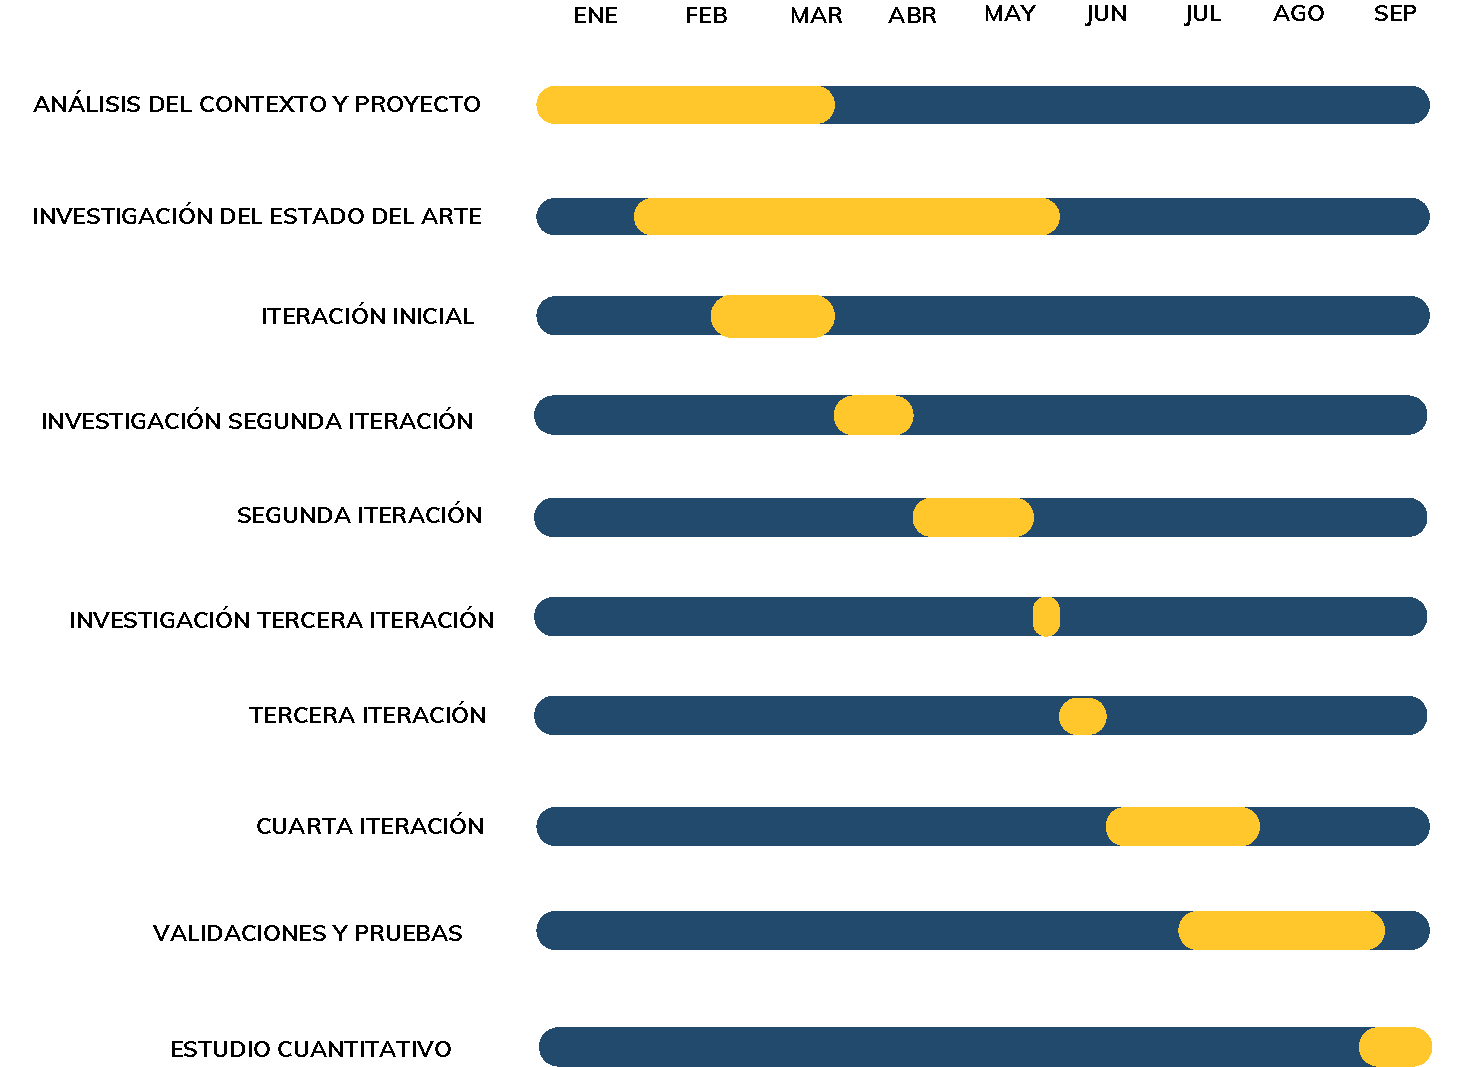
\includegraphics[scale= 0.5]{imagenes/1 ene - 25 MAR.pdf}
    \captionsetup{justification=centering}
    \caption{Diagrama de Gantt}
    \label{Diagrama de Gantt}
\end{figure}

\subsection{Presupuesto:}
Esta sección contiene el desglose de los diversos recursos, humanos y
materiales, usados durante el desarrollo del proyecto, incluyendo al final la
suma de los costes totales.

\subsubsection{Costes de Personal}
Los primeros costes a tener en cuenta son los del personal, en el se incluyen
las horas de trabajo del alumno junto con las de tutorías y de trabajo por parte
del tutor, que en este caso toma el papel de director del proyecto. El total de
horas que corresponden al trabajo por parte del alumno son 375, originadas del
número de créditos asignados al proyecto, siendo estos un total de 12 y
equivaliendo cada uno a 31,25 horas de trabajo se llega a esta cifra final. El
coste total de personal se obtiene multiplicando el número de horas finales por
los sueldos estándares de cada rol, siendo estos 15€/hora en el caso de un
ingeniero y de 50€/h en el caso del director.

\begin{table}[H]
    \centering
    \begin{tabular}{|c|c|c|c|}
        \hline
        \textbf{Cargo} & \textbf{Horas} & \textbf{Coste por hora} & \textbf{Coste Total} \\
        \hline
        Ingeniero             & 375 & 15€/hora & 5.625€ \\ \hline
        Director del Proyecto & 25  & 50€/hora & 750€   \\ \hline
        Total                 &     &          & 6.375€ \\ \hline
    \end{tabular}
    \caption{Tabla costes de personal.}
    \label{tab:03_29}
\end{table}


\subsubsection{Costes Software y Hardware}
Los costes relacionados con el software y hardware utilizados son los
siguientes, teniendo en cuenta la compra de un portátil (HP Pavilion Notebook
15-bc5) al inicio de la carrera, el gasto parcial de este será el
correspondiente a los 4 meses de trabajo dentro de los 4 años totales de uso. El
resto de gastos de hardware y software son 0 debido al uso de herramientas y
software \textit{open-source} y a los beneficios obtenidos por ser estudiante, los cuales
proporcionan multitud de licencias gratis. 

\begin{table}[H]
    \centering
    \begin{tabular}{|c|c|c|c|c|c|}
        \hline
        \textbf{Producto} & \textbf{Coste} & \textbf{Amortización}&
        \textbf{Coste por mes}& \textbf{Uso en proyecto}& \textbf{Coste Total}\\
        \hline

        Portátil          & 500€   & 48 meses & $10,41\frac{\textrm{\officialeuro}}{mes}$ & 4 meses & 41,64€ \\ \hline
        VisualStudio Code & 0      & -        & -                                         & -       & 0      \\ \hline
        Python            & 0      & -        & -                                         & -       & 0      \\ \hline
        Windows           & 0      & -        & -                                         & -       & 0      \\ \hline
        Total             & -      & -        & -                                         & -       & 41,64€ \\ \hline
    \end{tabular}
    \caption{Tabla costes de software y hardware.}
    \label{tab:03_30}
\end{table}

\subsubsection{Costes Indirectos}
Los costes indirectos son aquellos que corresponden a los recursos no
materiales utilizados durante el proyecto, estos incluyen la electricidad e
internet usados.
\begin{table}[H]
    \centering
    \begin{tabular}{|c|c|c|c|}
        \hline
        \textbf{Producto} & \textbf{Precio por Mes} & \textbf{Uso en Proyecto} & \textbf{Coste Total}  \\ \hline
        Electricidad         & 50€  & 6 meses  & 300€ \\ \hline
        Servicio de Internet & 30€  & 6 meses  & 180€ \\ \hline
        Total                &      &          & 480€ \\ \hline
    \end{tabular}
    \caption{Tabla costes indirectos.}
    \label{tab:03_31}

\end{table}

Finalmente se incluyen los costes totales, donde se agrupan todos los anteriores
para generar un presupuesto final del proyecto.
\begin{table}[H]
\centering
\begin{tabular}{|c|c|}
\hline
\textbf{Producto} & \textbf{Gasto Total} \\\hline
Personal          & 6.375€  \\\hline
Material          & 41,64€    \\\hline
Costes indirectos & 480€    \\\hline
Total             & 6.896.64€  \\\hline

\end{tabular}
  \caption{Tabla costes totales.}
  \label{tab:03_32}
\end{table}

\section{Impacto socio-económico} 
El desarrollo de este proyecto tiene un potencial impacto
socio-económico considerable. Este impacto se extiende a varias áreas críticas y
se encuentra en consonancia con los esfuerzos globales hacia la sostenibilidad,
tal como lo establece la Agenda 2030 de las Naciones Unidas. En este contexto,
la asignación automatizada de \gls{ODSa} a textos puede ser vista como un valioso
recurso para mejorar la eficiencia en la gestión y la toma de decisiones, así
como para promover la conciencia y la acción en torno a los \gls{ODSa}.

En primer lugar, este tipo de proyecto respalda directamente la Agenda de
Desarrollo Sostenible de las Naciones Unidas, que establece 17 \gls{ODSa} para abordar
problemas globales como la pobreza, el hambre, la igualdad de género, la acción
climática y la paz y la justicia. Al asignar los \gls{ODSa} de manera automatizada a
documentos y textos relacionados, el proyecto facilita la alineación de
esfuerzos y recursos hacia la consecución de estos objetivos, contribuyendo así
al progreso global hacia un futuro sostenible.

Además, la asignación automatizada de \gls{ODSa} a textos puede tener un impacto
significativo en la toma de decisiones informadas. Al identificar de manera
eficiente y precisa la relevancia de los contenidos de texto en relación con los
\gls{ODSa}, las organizaciones y los responsables de la toma de decisiones pueden
contar con una herramienta valiosa para evaluar la coherencia y la contribución
de sus acciones y políticas a los objetivos de sostenibilidad. Esta mejora en la
capacidad de toma de decisiones puede tener repercusiones positivas tanto en el
sector público como en el privado.


%---------------------------------
%---------------------------------
En el contexto de la investigación científica, la aplicación de sistemas de
clasificación automatizada de textos emerge como una herramienta de gran
relevancia para agilizar y optimizar la revisión de la literatura relacionada
con los \gls{ODSg} (\gls{ODSa}). Esta tecnología posee el
potencial de reducir de manera significativa el tiempo invertido por los
investigadores en la búsqueda, selección y análisis de documentos relacionados
con los \gls{ODSa}, lo que a su vez conduce a una mejora palpable en la calidad y
eficiencia de la investigación en los campos asociados a la sostenibilidad.

La capacidad de estos sistemas de identificar y categorizar de manera rápida y
precisa los documentos que abordan aspectos relevantes de los \gls{ODSa}, proporciona
una ventaja sustancial en la identificación de áreas específicas que requieren
una mayor atención y dedicación de recursos. Esto permite una asignación más
efectiva de recursos humanos y financieros, facilitando la priorización de
investigaciones en los ámbitos que requieren una mayor atención en términos de
estudios o que presentan un mayor potencial de impacto en la consecución de los
\gls{ODSa}.
%---------------------------------
%---------------------------------

Desde una perspectiva más amplia, la aplicación de modelos de asignación
automatizada de Objetivos de Desarrollo Sostenible \gls{ODSa} a textos no solo
influye en la toma de decisiones políticas y estratégicas al proporcionar datos
cuantitativos para identificar áreas de investigación prioritarias, sino que
también puede tener un impacto significativo en la conciencia pública y la
adopción de prácticas sostenibles. Al etiquetar y resaltar contenido relacionado
con los \gls{ODSa}, se puede fomentar una mayor comprensión y compromiso con los
problemas y desafíos que abordan estos objetivos. Esto, a su vez, puede influir
en las decisiones individuales y colectivas, así como en la forma en que las
instituciones, publicas y privadas, abordan las cuestiones de sostenibilidad en
sus operaciones económicas y políticas.
%---------------------------------
%---------------------------------

Desde una perspectiva económica, este proyecto, se anticipa que tenga un impacto
económico mínimo, cercano a cero, ya que no se enfoca en objetivos comerciales
explícitos como la monetización del modelo. Su principal valor radica en su
utilidad para la investigación y el análisis de los \gls{ODSg} (\gls{ODSa}) al automatizar el procesamiento y la clasificación de textos.
Es este último aspecto el que puede tener cierto impacto económico, aunque
limitado, pudiendo llegar a reducir el tiempo necesario para tratar textos,
ayudando a alocar recursos económicos en otras áreas de interés.  

En resumen, este proyecto puede tener un impacto socio-económico positivo y
significativo. Esto se manifiesta en la promoción de la sostenibilidad, la
mejora de la toma de decisiones, la eficiencia en la investigación científica,
la generación de conocimiento y la promoción de la responsabilidad gubernamental
y empresarial. Además, este proyecto se alinea con los objetivos globales de
desarrollo sostenible y contribuye al avance de la Agenda 2030 de las Naciones
Unidas.

